\documentclass{beamer}

\usefonttheme{professionalfonts} % using non standard fonts for beamer
\usefonttheme{serif} % default family is serif

\usepackage{hyperref}
%\usepackage{minted}
\usepackage{animate}
\usepackage{graphicx}
\def\Put(#1,#2)#3{\leavevmode\makebox(0,0){\put(#1,#2){#3}}}
\usepackage{colortbl}
\usepackage{tikz}
\usepackage{amssymb}
\usepackage{enumerate}
\usepackage{arydshln}
\usepackage{algorithm}
\usepackage{algpseudocode}

\colorlet{lightred}{red!25}
\colorlet{lightgreen}{green!25}


\newcommand\blfootnote[1]{%

  \begingroup

  \renewcommand\thefootnote{}\footnote{#1}%

  \addtocounter{footnote}{-1}%

  \endgroup

}

\makeatletter

%%%%%%%%%%%%%%%%%%%%%%%%%%%%%% Textclass specific LaTeX commands.

 % this default might be overridden by plain title style

 \newcommand\makebeamertitle{\frame{\maketitle}}%

 % (ERT) argument for the TOC

 \AtBeginDocument{%

   \let\origtableofcontents=\tableofcontents

   \def\tableofcontents{\@ifnextchar[{\origtableofcontents}{\gobbletableofcontents}}

   \def\gobbletableofcontents#1{\origtableofcontents}

 }

%%%%%%%%%%%%%%%%%%%%%%%%%%%%%% User specified LaTeX commands.

\usetheme{Malmoe}

% or ...

\useoutertheme{infolines}

\addtobeamertemplate{headline}{}{\vskip2pt}

\setbeamercovered{transparent}

% or whatever (possibly just delete it)

\makeatother

\begin{document}
\title[PFLOCK report]{PFLOCK Report}
\author[AC]{Andres Calderon}
\institute[Winter'20]{University of California, Riverside}
\makebeamertitle
\newif\iflattersubsect

\AtBeginSection[] {
    \begin{frame}<beamer>
    \frametitle{Outline} 
    \tableofcontents[currentsection]  
    \end{frame}
    \lattersubsectfalse
}

\AtBeginSubsection[] {
    \begin{frame}<beamer>
    \frametitle{Outline} 
    \tableofcontents[currentsubsection]  
    \end{frame}
}


\begin{frame}{What was the problem?}
    \begin{itemize}
        \item Apache Spark do not preserve partitioning by default. It has to be done explicitly in some operation such as MapPartitions, which are usually use in Joins.
        \item GeoSpark uses a \textit{mapToPair} function which does not allow to set the parameter \textit{preservesPartitioning}\footnote{\tiny \url{http://apache-spark-user-list.1001560.n3.nabble.com/preservesPartitioning-td10019.html}}.
        \item In the new implementation in Scala it is easier to force this parameter to True during a \textit{MapPartitions} operation.
    \end{itemize}
\end{frame}

\begin{frame}{Solving distance join issue in GeoSpark...}{Pointset A}
    \centering
    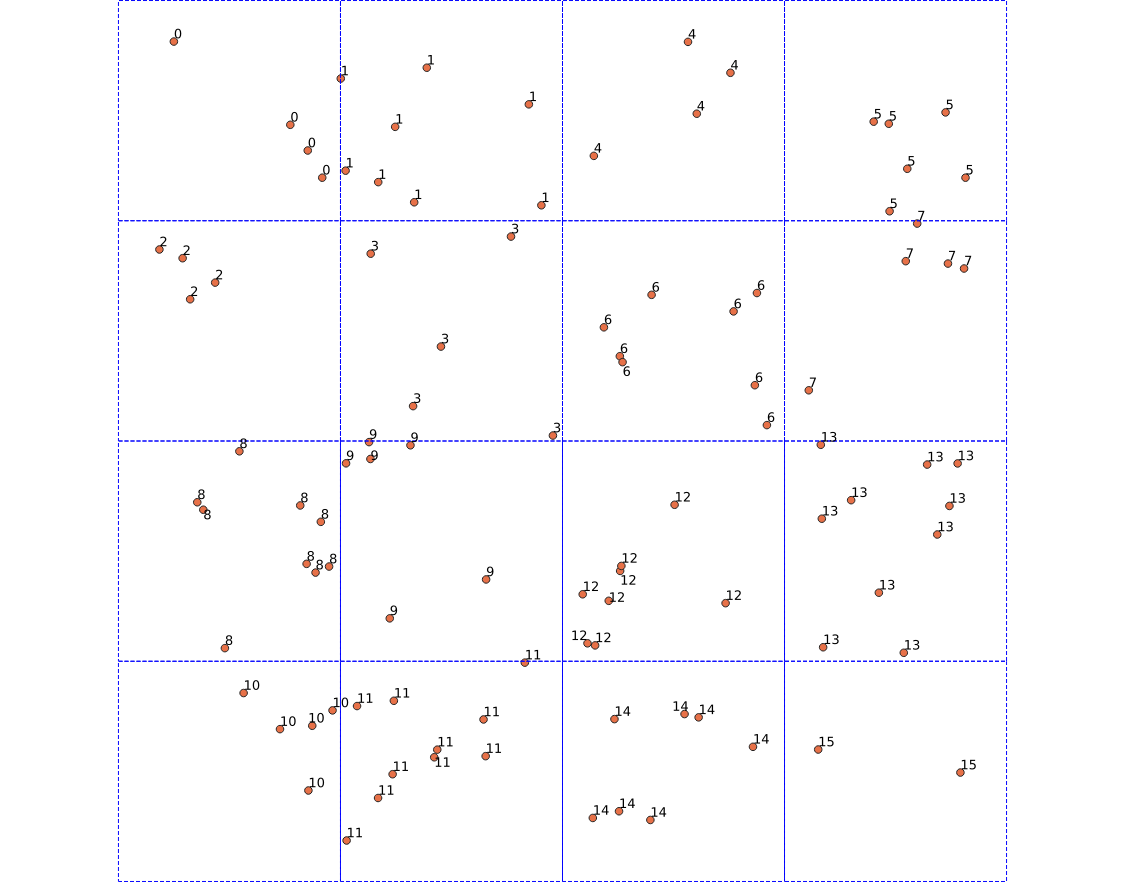
\includegraphics[width=0.8\textwidth]{figures/points}
\end{frame}
\begin{frame}{Solving distance join issue in GeoSpark...}{Pointset B}
    \centering
    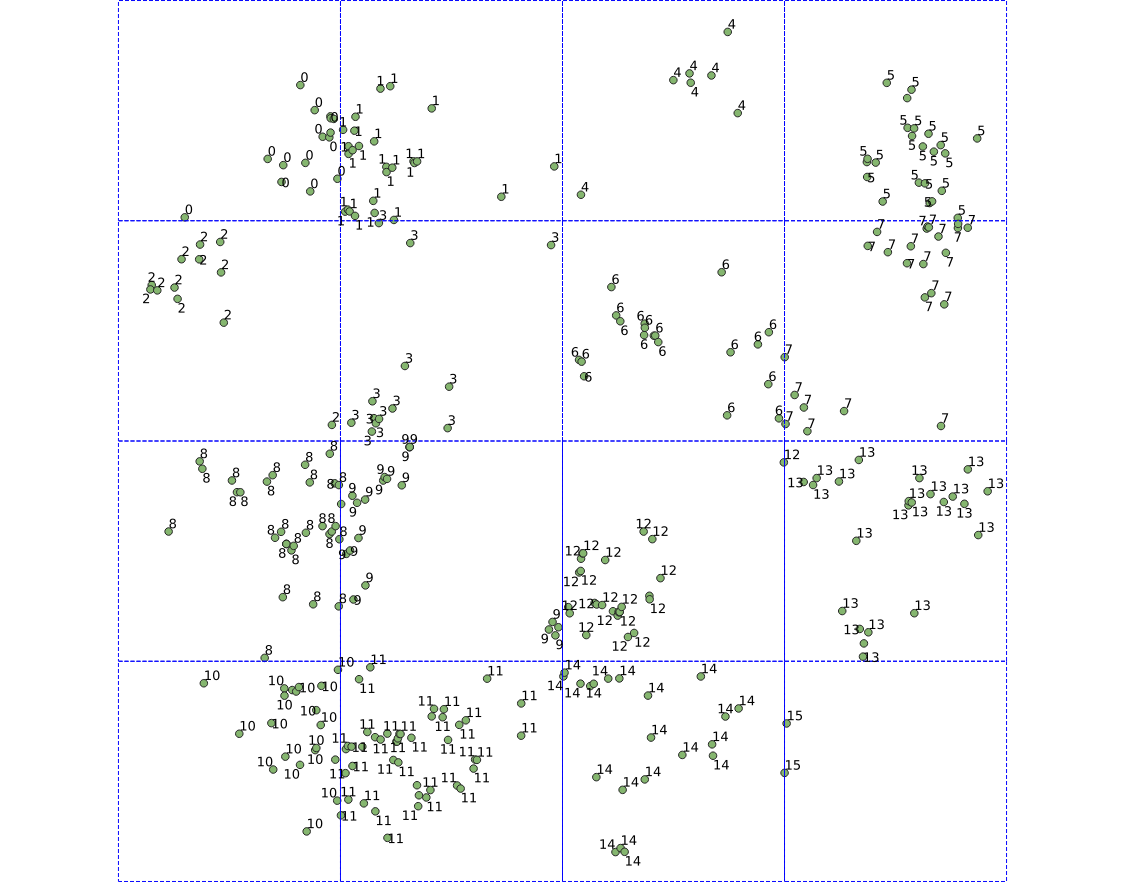
\includegraphics[width=0.8\textwidth]{figures/centers}
\end{frame}
\begin{frame}{Solving distance join issue in GeoSpark...}{Previous}
    \centering
    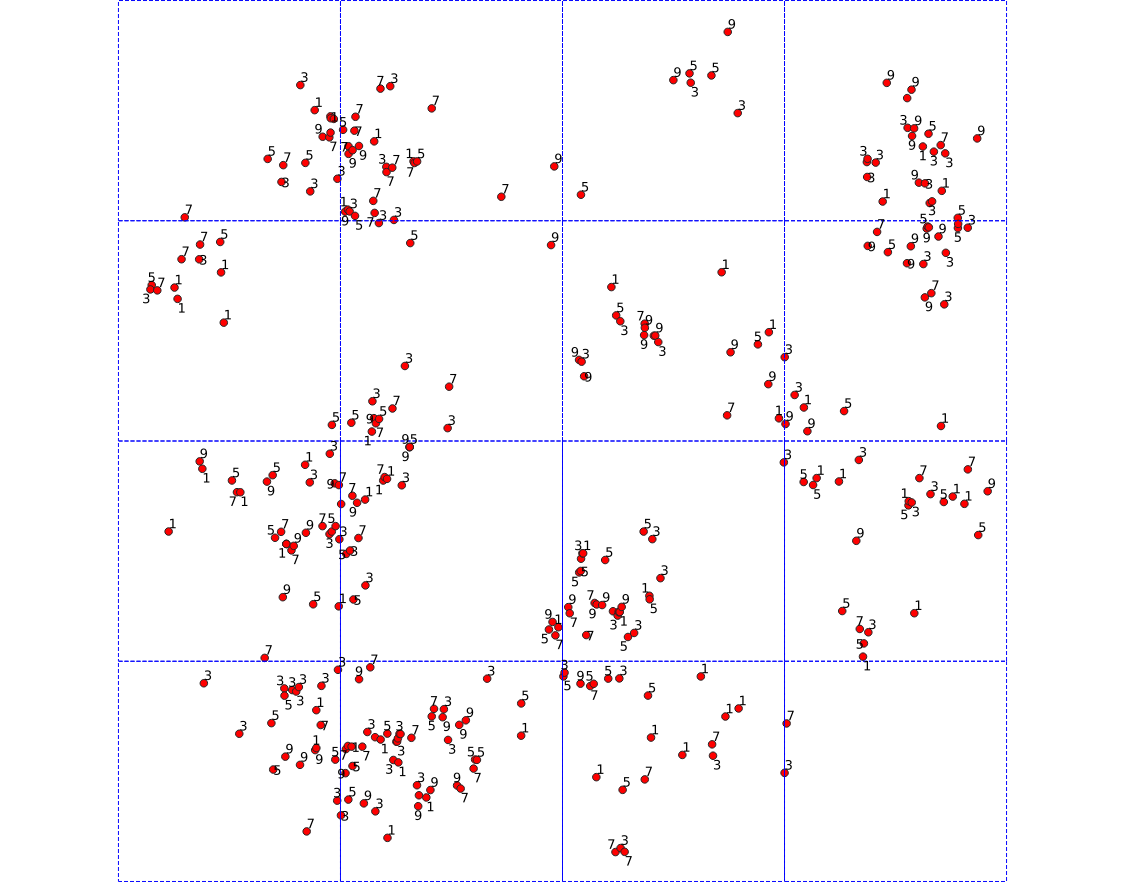
\includegraphics[width=0.8\textwidth]{figures/geospark}
\end{frame}
\begin{frame}{Solving distance join issue in GeoSpark...}{Current}
    \centering
    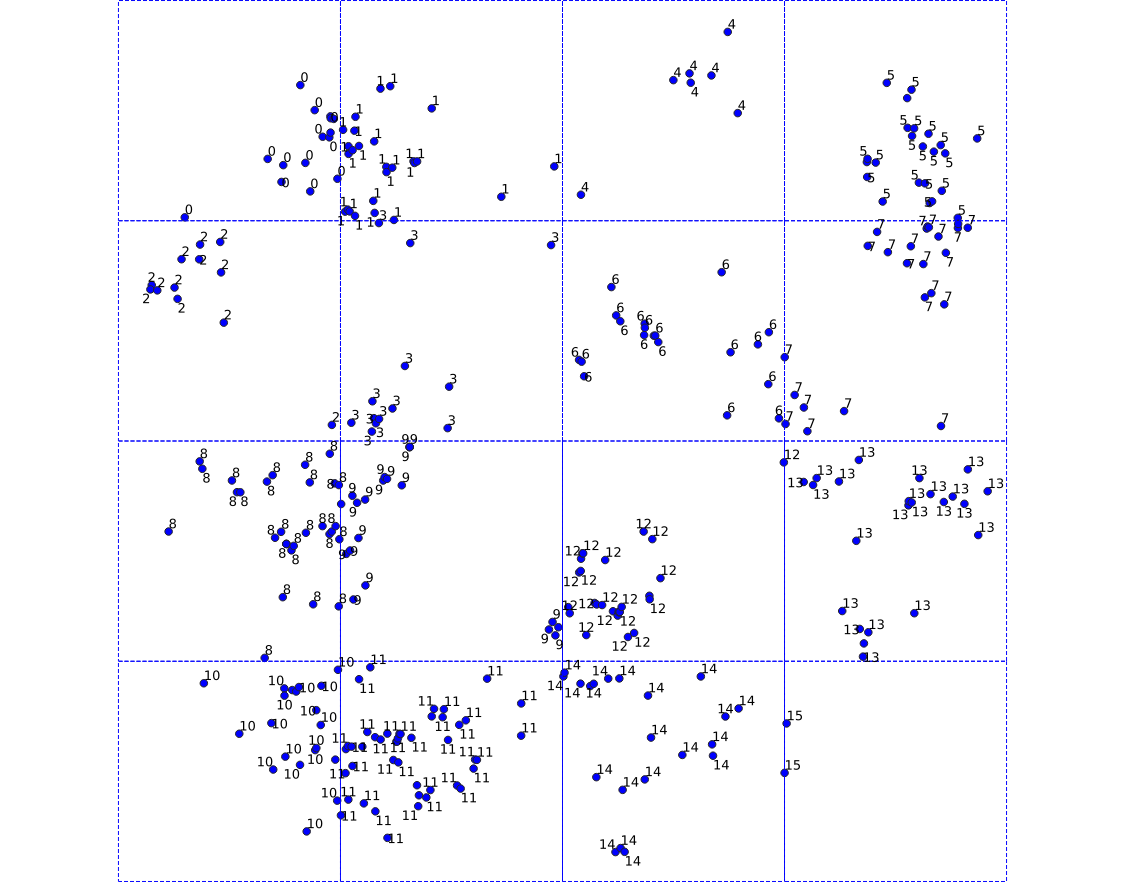
\includegraphics[width=0.8\textwidth]{figures/new}
\end{frame}

\begin{frame}{What's next?}
    \begin{itemize}
        \item Currently working on the new partition-based indexing implementation.
        \item Implement the new changes in the previous code.
    \end{itemize}
\end{frame}

\end{document}
